% ==============================================================================
% =================================== Aufgabe 3 ================================
% ==============================================================================

\chapter{Aufgabe (3)}
\label{chap:Aufgabe3}
\thispagestyle{fancy}

Die folgende Aufgabe basiert auf dem \texttt{Wine}-Datensatz aus der Bibliothek \texttt{sklearn.datasets}. Der Datensatz enthält die Ergebnisse einer chemischen Analyse von Weinen, die in derselben Region in Italien von drei verschiedenen Weinbauern angebaut wurden. Es gibt dreizehn verschiedene Messungen für verschiedene Bestandteile, die in den drei Weinsorten vorkommen.

% ======================================= a =====================================

\section{Bibliotheken importieren, Datensatz laden – Typen von wine, wine.data und wine.target (a)}
\label{sec:3a}

\subsection{Aufgabenstellung}

Die erforderlichen Bibliotheken werden importiert und der \texttt{Wine}-Datensatz wird geladen. Die Typen von \texttt{wine}, \texttt{wine.data} und \texttt{wine.target} werden ermittelt und beschrieben.

\subsection{Lösung}

Der \texttt{Wine}-Datensatz wird mit der Funktion \texttt{load\_wine()} aus \texttt{sklearn.datasets} geladen. Der Parameter \texttt{as\_frame=True} sorgt dafür, dass die Daten als \texttt{Pandas DataFrame} zurückgegeben werden. Die Typen der einzelnen Komponenten werden mit \texttt{type()} ermittelt.

\lstinputlisting[
    language=Python,
    caption={Bibliotheken importieren, Datensatz laden und Typen prüfen},
    label={lst:aufgabe3a}
]{asset/code/Aufgabe3a.tex}

\subsection{Ausgabe}

Die Ausgabe zeigt die Typen der einzelnen Komponenten:

\begin{verbatim}
Typ von wine: <class 'sklearn.utils._bunch.Bunch'>
Typ von wine.data: <class 'pandas.DataFrame'>
Typ von wine.target: <class 'pandas.Series'>

Erste 5 Zeilen von wine.data:
   alcohol  malic_acid   ash  alcalinity_of_ash  magnesium  total_phenols  \
0    14.23        1.71  2.43               15.6      127.0           2.80   
1    13.20        1.78  2.14               11.2      100.0           2.65   
2    13.16        2.36  2.67               18.6      101.0           2.80   
3    14.37        1.95  2.50               16.8      113.0           3.85   
4    13.24        2.59  2.87               21.0      118.0           2.80   

   flavanoids  nonflavanoid_phenols  proanthocyanins  color_intensity   hue  \
0        3.06                  0.28             2.29             5.64  1.04   
1        2.76                  0.26             1.28             4.38  1.05   
2        3.24                  0.30             2.81             5.68  1.03   
3        3.49                  0.24             2.18             7.80  0.86   
4        2.69                  0.39             1.82             4.32  1.04   

   od280/od315_of_diluted_wines  proline  
0                          3.92   1065.0  
1                          3.40   1050.0  
2                          3.17   1185.0  
3                          3.45   1480.0  
4                          2.93    735.0  

Erste 5 Werte von wine.target:
0    0
1    0
2    0
3    0
4    0
Name: target, dtype: int64

Feature names: ['alcohol', 'malic_acid', 'ash', 'alcalinity_of_ash', 'magnesium', 'total_phenols', 'flavanoids', 'nonflavanoid_phenols', 'proanthocyanins', 'color_intensity', 'hue', 'od280/od315_of_diluted_wines', 'proline']
Target names: ['class_0' 'class_1' 'class_2']
Data shape: (178, 13)
\end{verbatim}

\subsection{Interpretation}

Der \texttt{Wine}-Datensatz wird mit \texttt{load\_wine(\textit{as\_frame=True})} geladen. Durch den Parameter \texttt{as\_frame=True} werden die Daten als \texttt{Pandas DataFrame} (\textit{\texttt{wine.data}}) und die Zielvariable als \texttt{Pandas Series} (\textit{\texttt{wine.target}}) zurückgegeben.

Die Typen der Komponenten sind:

\begin{itemize}
    \item \texttt{wine}: Ein \texttt{Bunch}-Objekt (\textit{dictionary-ähnliche Datenstruktur aus \texttt{sklearn}}), das die Daten, die Zielvariable, die Feature-Namen und die Ziel-Namen enthält.
    \item \texttt{wine.data}: Ein \texttt{Pandas DataFrame} mit 13 numerischen Spalten (\textit{den chemischen Messungen}) und 178 Zeilen (\textit{den Weinproben}).
    \item \texttt{wine.target}: Eine \texttt{Pandas Series} mit den Klassenlabels (\textit{0, 1, 2}) für die drei verschiedenen Weinsorten.
\end{itemize}

Der \texttt{Wine}-Datensatz enthält 178 Instanzen und 13 Attribute. Die Zielvariable besteht aus drei Klassen, die die drei verschiedenen Weinbauern repräsentieren.

\cleardoublepage

% ======================================= b =====================================

\section{Countplot für wine.target (b)}
\label{sec:3b}

\subsection{Aufgabenstellung}

Es wird ein Countplot für die Zielvariable \texttt{wine.target} erstellt, um die Verteilung der drei Weinsorten zu visualisieren.

\subsection{Lösung}

Der Countplot wird mit der Funktion \texttt{sns.countplot()} aus der Bibliothek \texttt{seaborn} erstellt. Die Zielvariable \texttt{wine.target} wird auf der x-Achse abgetragen. Die Plot-Größe wird mit \texttt{plt.figure(\textit{figsize=(8,6)})} angepasst. Die Achsen werden beschriftet, um die Lesbarkeit zu verbessern.

\lstinputlisting[
    language=Python,
    caption={Countplot für wine.target},
    label={lst:aufgabe3b}
]{asset/code/Aufgabe3b.tex}

\subsection{Ausgabe}

Die Ausgabe zeigt die Häufigkeitsverteilung der drei Weinsorten:

\begin{figure}[h]
    \centering
    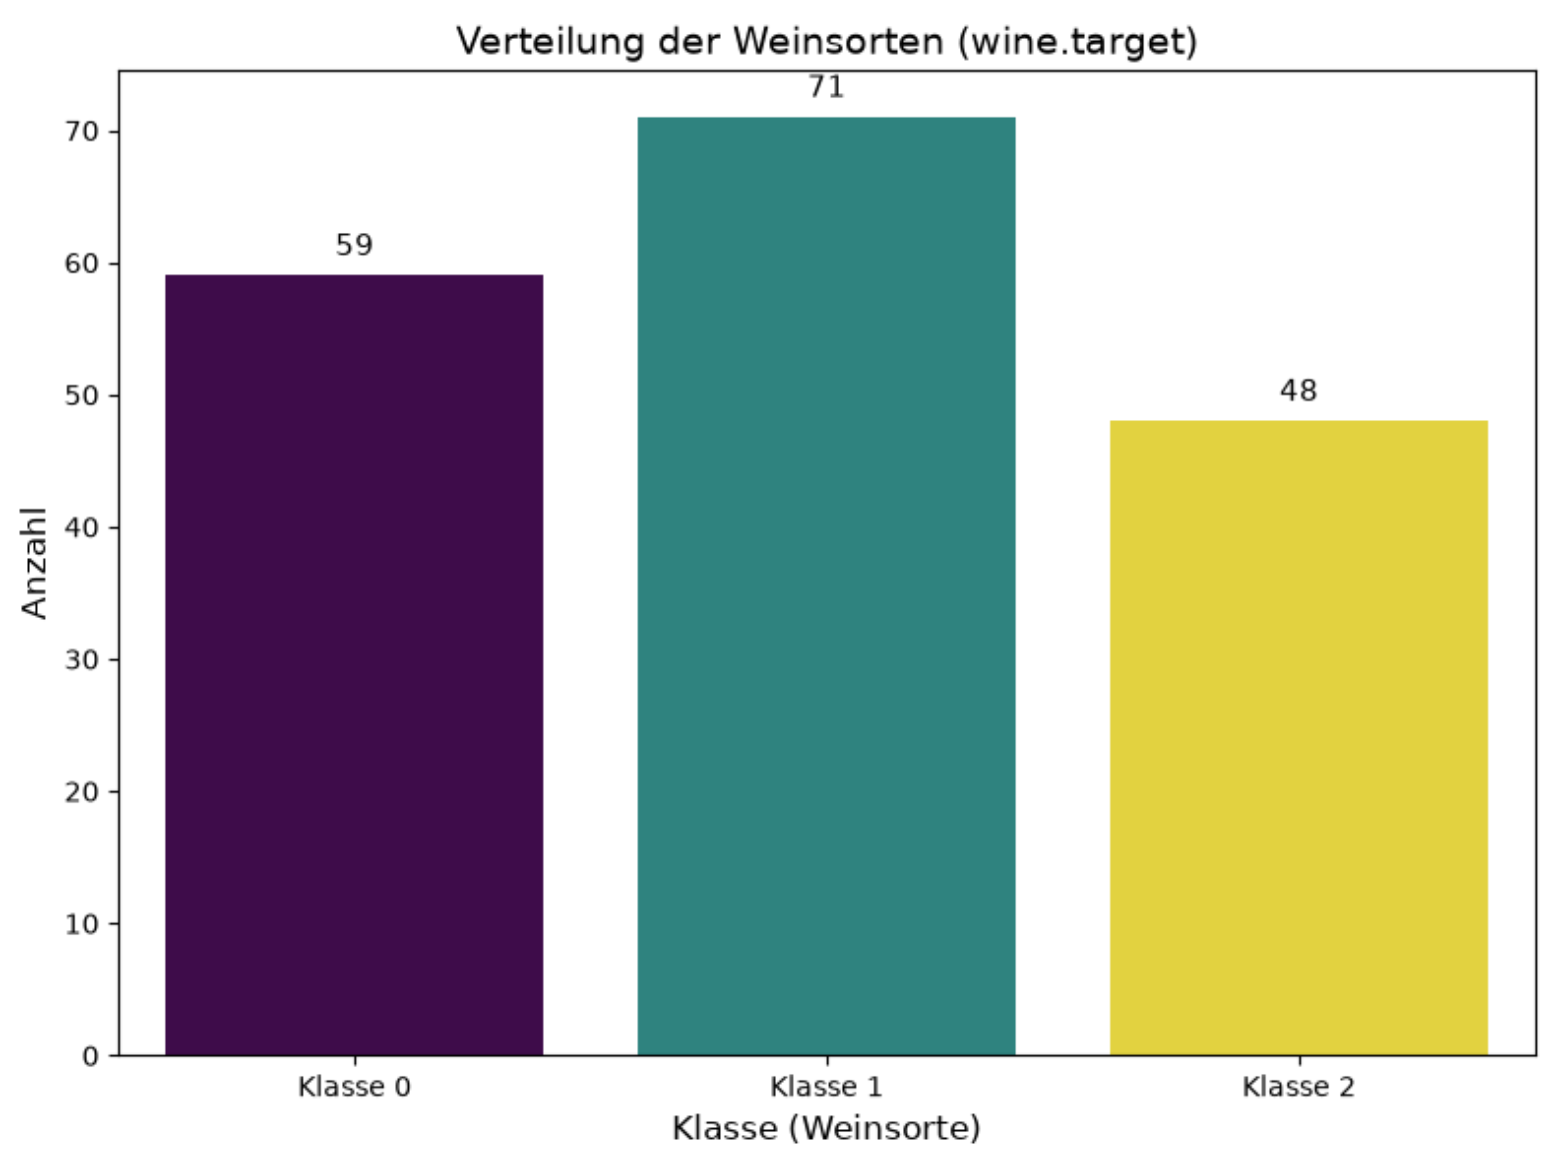
\includegraphics[width=0.9\textwidth]{./asset/image/Aufgabe3b.png}
    \caption{Countplot für wine.target (\textit{Quelle: Eigene Darstellung})}
    \label{fig:aufgabe3b}
\end{figure}

\subsection{Interpretation}

Der Countplot wird mit \texttt{sns.countplot(\textit{x=wine.target})} erstellt. Die Zielvariable \texttt{wine.target} enthält die Klassenlabels 0, 1 und 2, die die drei verschiedenen Weinbauern repräsentieren. Der Plot zeigt die Anzahl der Weinproben pro Klasse.

Die Verteilung der drei Klassen ist relativ ausgeglichen. Jede Klasse enthält etwa 60 Proben, was auf eine ausgewogene Stichprobe hinweist. Dies ist vorteilhaft für die spätere Klassifikation, da keine Klasse überrepräsentiert ist.

\cleardoublepage

% ======================================= c =====================================

\section{Summenstatistik von wine.data und größte Standardabweichung (c)}
\label{sec:3c}

\subsection{Aufgabenstellung}

Es wird eine Summenstatistik des Datensatzes \texttt{wine.data} erstellt. Es wird ermittelt, welche Variable die größte Standardabweichung aufweist.

\subsection{Lösung}

Die Summenstatistik wird mit der Methode \texttt{describe()} auf dem \texttt{DataFrame} \texttt{wine.data} berechnet. Die Standardabweichungen der einzelnen Variablen werden mit \texttt{std()} berechnet. Die Variable mit der größten Standardabweichung wird mit \texttt{idxmax()} ermittelt.

\lstinputlisting[
    language=Python,
    caption={Summenstatistik von wine.data und Ermittlung der größten Standardabweichung},
    label={lst:aufgabe3c}
]{asset/code/Aufgabe3c.tex}

\subsection{Ausgabe}

Die Ausgabe zeigt die Summenstatistik des Datensatzes sowie die Variable mit der größten Standardabweichung:

\begin{verbatim}
Summenstatistik von wine.data:
          alcohol  malic_acid         ash  alcalinity_of_ash   magnesium  \
count  178.000000  178.000000  178.000000         178.000000  178.000000   
mean    13.000618    2.336348    2.366517          19.494944   99.741573   
std      0.811827    1.117146    0.274344           3.339564   14.282484   
min     11.030000    0.740000    1.360000          10.600000   70.000000   
25%     12.362500    1.602500    2.210000          17.200000   88.000000   
50%     13.050000    1.865000    2.360000          19.500000   98.000000   
75%     13.677500    3.082500    2.557500          21.500000  107.000000   
max     14.830000    5.800000    3.230000          30.000000  162.000000   

       total_phenols  flavanoids  nonflavanoid_phenols  proanthocyanins  \
count     178.000000  178.000000            178.000000       178.000000   
mean        2.295112    2.029270              0.361854         1.590899   
std         0.625851    0.998859              0.124453         0.572359   
min         0.980000    0.340000              0.130000         0.410000   
25%         1.742500    1.205000              0.270000         1.250000   
50%         2.355000    2.135000              0.340000         1.555000   
75%         2.800000    2.875000              0.437500         1.950000   
max         3.880000    5.080000              0.660000         3.580000   

       color_intensity         hue  od280/od315_of_diluted_wines      proline  
count       178.000000  178.000000                    178.000000   178.000000  
mean          5.058090    0.957449                      2.611685   746.893258  
std           2.318286    0.228572                      0.709990   314.907474  
min           1.280000    0.480000                      1.270000   278.000000  
25%           3.220000    0.782500                      1.937500   500.500000  
50%           4.690000    0.965000                      2.780000   673.500000  
75%           6.200000    1.120000                      3.170000   985.000000  
max          13.000000    1.710000                      4.000000  1680.000000  

Die Variable mit der größten Standardabweichung ist: proline (314.91)
\end{verbatim}

Die Standardabweichungen aller Variablen (\textit{absteigend sortiert}):

\begin{verbatim}
Standardabweichungen aller Variablen (absteigend sortiert):
proline                         314.907474
magnesium                        14.282484
alcalinity_of_ash                 3.339564
color_intensity                   2.318286
malic_acid                        1.117146
flavanoids                        0.998859
alcohol                           0.811827
od280/od315_of_diluted_wines      0.709990
total_phenols                     0.625851
proanthocyanins                   0.572359
ash                               0.274344
hue                               0.228572
nonflavanoid_phenols              0.124453
dtype: float64
\end{verbatim}

\subsection{Interpretation}

Die Summenstatistik wird mit \texttt{wine.data.describe()} berechnet. Sie zeigt für jede der 13 Variablen die wichtigsten statistischen Kennzahlen: Anzahl, Mittelwert, Standardabweichung, Minimum, 25\%-Quantil, Median, 75\%-Quantil und Maximum.

Die Variable mit der größten Standardabweichung ist \texttt{proline} mit einem Wert von etwa 314.91. Dies bedeutet, dass die Prolin-Konzentration in den Weinproben die größte Variationsbreite aufweist. Auch \texttt{magnesium} (\textit{14.28}) und \texttt{alcalinity\_of\_ash} (\textit{3.34}) zeigen hohe Standardabweichungen. Die Variable \texttt{nonflavanoid\_phenols} zeigt mit etwa 0.124 die geringste Standardabweichung, was auf eine relativ konstante Konzentration in den Weinen hinweist.

Die großen Unterschiede in den Standardabweichungen (\textit{von 0.124 bis 314.91}) sind ein deutlicher Hinweis darauf, dass eine Skalierung der Daten für bestimmte Machine-Learning-Verfahren (\textit{\acs{z. B.} K-Means-Clustering}) erforderlich sein könnte. Variablen mit großen Wertebereichen wie \texttt{proline} würden sonst einen unverhältnismäßig großen Einfluss auf die Distanzberechnung haben und die Clusterbildung verzerren.

\cleardoublepage

% ======================================= d =====================================

\section{Korrelationsplot (d)}
\label{sec:3d}

\subsection{Aufgabenstellung}

Es wird ein Korrelationsplot für \texttt{wine.data} erstellt. Es wird ermittelt, welche Variablen am stärksten korreliert sind.

\subsection{Lösung}

Die Korrelationsmatrix wird mit der Methode \texttt{corr()} auf dem \texttt{DataFrame} \texttt{wine.data} berechnet. Der Korrelationsplot wird mit \texttt{sns.heatmap()} visualisiert. Die stärksten Korrelationen werden durch Analyse der Korrelationsmatrix ermittelt.

\lstinputlisting[
    language=Python,
    caption={Korrelationsplot für wine.data},
    label={lst:aufgabe3d}
]{asset/code/Aufgabe3d.tex}

\subsection{Ausgabe}

Die Ausgabe zeigt den Korrelationsplot sowie die stärksten Korrelationen:

\begin{figure}[h]
    \centering
    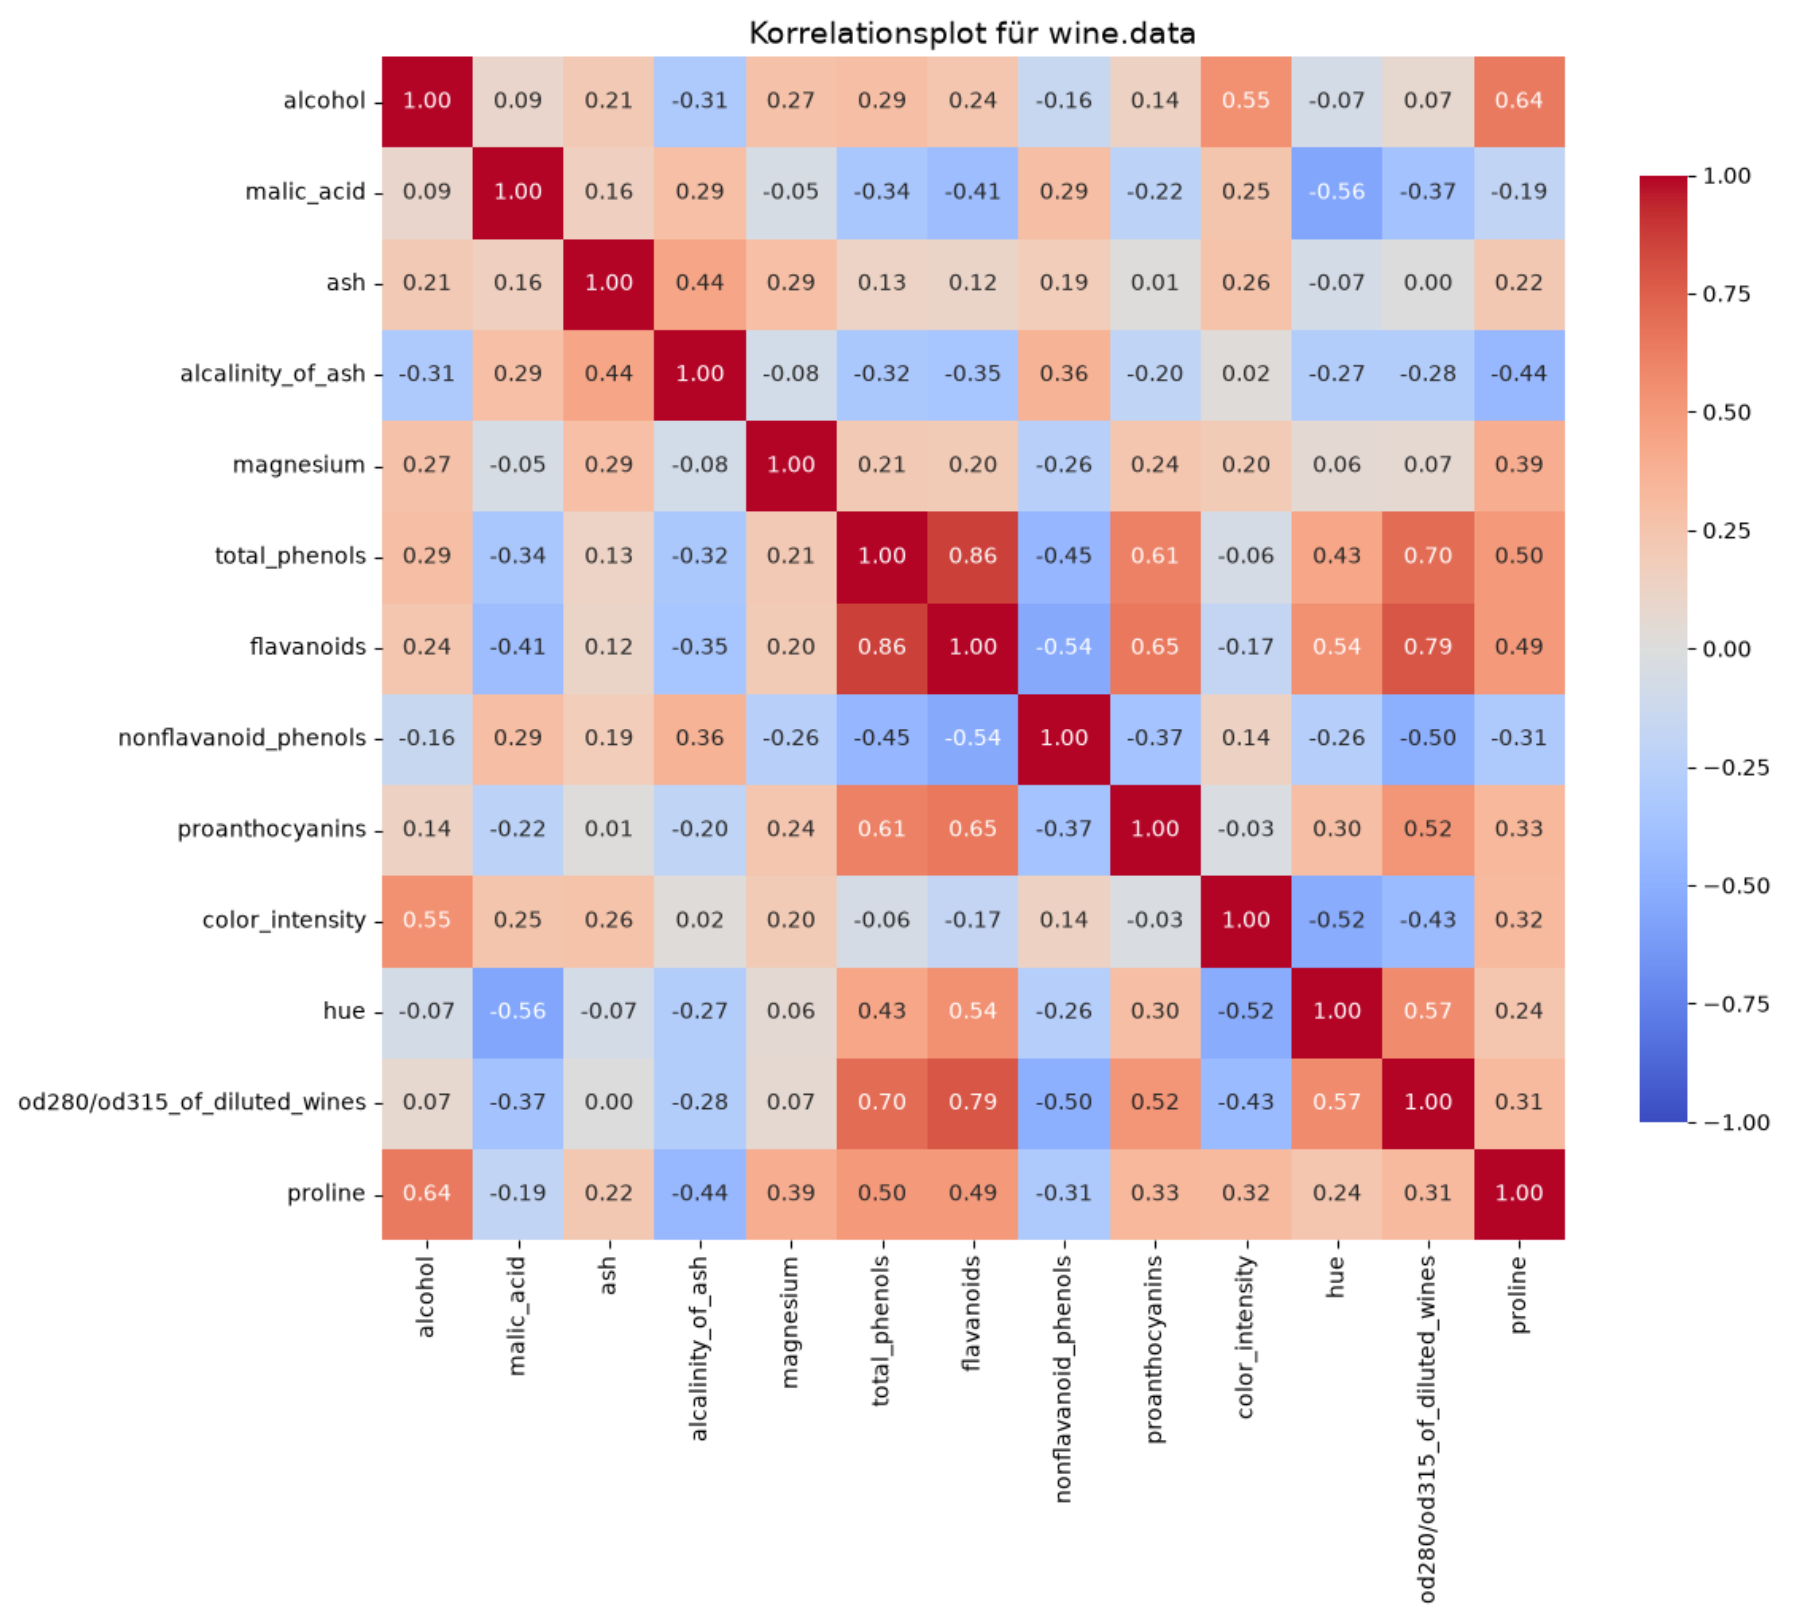
\includegraphics[width=0.9\textwidth]{./asset/image/Aufgabe3d.png}
    \caption{Korrelationsplot für wine.data (\textit{Quelle: Eigene Darstellung})}
    \label{fig:aufgabe3d}
\end{figure}

Die stärksten positiven Korrelationen im Datensatz sind:

\begin{verbatim}
Stärkste positive Korrelationen:
total_phenols    flavanoids                      0.864564
flavanoids       od280/od315_of_diluted_wines    0.787194
total_phenols    od280/od315_of_diluted_wines    0.699949
flavanoids       proanthocyanins                 0.652692
alcohol          proline                         0.643720
total_phenols    proanthocyanins                 0.612413
hue              od280/od315_of_diluted_wines    0.565468
alcohol          color_intensity                 0.546364
flavanoids       hue                             0.543479
proanthocyanins  od280/od315_of_diluted_wines    0.519067
dtype: float64
\end{verbatim}

Die stärksten negativen Korrelationen im Datensatz sind:

\begin{verbatim}
Stärkste negative Korrelationen:
malic_acid            hue                            -0.561296
flavanoids            nonflavanoid_phenols           -0.537900
color_intensity       hue                            -0.521813
nonflavanoid_phenols  od280/od315_of_diluted_wines   -0.503270
total_phenols         nonflavanoid_phenols           -0.449935
alcalinity_of_ash     proline                        -0.440597
color_intensity       od280/od315_of_diluted_wines   -0.428815
malic_acid            flavanoids                     -0.411007
                      od280/od315_of_diluted_wines   -0.368710
nonflavanoid_phenols  proanthocyanins                -0.365845
dtype: float64
\end{verbatim}

\subsection{Interpretation}

Die Korrelationsmatrix wird mit \texttt{wine.data.corr()} berechnet. Der Korrelationsplot mit \texttt{sns.heatmap()} visualisiert die paarweisen Korrelationen zwischen allen 13 Variablen. Die Farbkodierung reicht von Blau (\textit{negative Korrelation}) über Weiß (\textit{keine Korrelation}) bis Rot (\textit{positive Korrelation}).

Die stärkste positive Korrelation besteht zwischen \texttt{total\_phenols} und \texttt{flavanoids} mit einem Korrelationskoeffizienten von etwa 0.865. Dies deutet darauf hin, dass Weine mit einem hohen Gehalt an Gesamtphenolen auch einen hohen Gehalt an Flavonoiden aufweisen. Ebenfalls stark positiv korreliert sind \texttt{flavanoids} und \\ \texttt{od280/od315\_of\_diluted\_wines} (\textit{0.787}) sowie \texttt{total\_phenols} und \texttt{od280/od315\_of\_diluted\_wines} (\textit{0.700}).

Die stärkste negative Korrelation besteht zwischen \texttt{malic\_acid} und \texttt{hue} mit etwa -0.561. Dies bedeutet, dass Weine mit höherem Maliksäuregehalt tendenziell eine geringere Farbintensität aufweisen. Ebenfalls negativ korreliert sind \texttt{flavanoids} und \texttt{nonflavanoid\_phenols} (\textit{-0.538}) sowie \texttt{color\_intensity} und \texttt{hue} (\textit{-0.522}).

Diese Korrelationen sind für die spätere Dimensionsreduktion und das Clustering relevant, da stark korrelierte Variablen redundante Informationen enthalten. Die starke Korrelation zwischen \texttt{total\_phenols} und \texttt{flavanoids} deutet darauf hin, dass diese beiden Variablen möglicherweise ähnliche Informationen über die Weinqualität liefern.

\cleardoublepage

% ======================================= e =====================================

\section{Kombinieren von wine.data und wine.target – Pairplot (e)}
\label{sec:3e}

\subsection{Aufgabenstellung}

Die Daten \texttt{wine.data} und die Zielvariable \texttt{wine.target} werden zu einem neuen Datensatz kombiniert. Es wird ein Pairplot erstellt. Es wird erklärt, welche Bedeutung die Graphen auf der Diagonalen des Pairplots haben. Es wird ermittelt, in welcher Zeile des Pairplots die Cluster am deutlichsten erkennbar sind.

\subsection{Lösung}

Zunächst werden \texttt{wine.data} und \texttt{wine.target} mit \texttt{pd.concat()} zu einem neuen \texttt{DataFrame} \texttt{wine\_df} kombiniert. Die Zielvariable wird als Spalte \texttt{target} hinzugefügt. Der Pairplot wird mit \texttt{sns.pairplot()} erstellt, wobei die Zielvariable als \texttt{hue} übergeben wird, um die drei Weinsorten farblich zu unterscheiden.

\lstinputlisting[
    language=Python,
    caption={Kombinieren der Daten und Erstellen des Pairplots},
    label={lst:aufgabe3e}
]{asset/code/Aufgabe3e.tex}

\subsection{Ausgabe}

Die Ausgabe zeigt den Pairplot des kombinierten Datensatzes:

\begin{verbatim}
Plot gespeichert als: ../output/Aufgabe3e.png
Vollständiger Pfad: C:\Users\USER\Downloads\B-BIDA01XX\output\Aufgabe3e.png
\end{verbatim}

\begin{figure}[h]
    \centering
    \includegraphics[width=0.9\textwidth]{./asset/image/Aufgabe3e.png}
    \caption{Pairplot des Wine-Datensatzes mit farblicher Kennzeichnung der drei Klassen (\textit{Quelle: Eigene Darstellung})}
    \label{fig:aufgabe3e}
\end{figure}

\subsection{Interpretation}

Der Pairplot wird mit \texttt{sns.pairplot(\textit{wine\_df}, \textit{hue='target'})} erstellt. Die drei Weinsorten (\textit{target = 0, 1, 2}) werden farblich unterschieden.

\textbf{Bedeutung der Diagonalen:}

Die Graphen auf der Diagonalen des Pairplots zeigen die Verteilung jeder einzelnen Variable, getrennt nach den drei Klassen. Es handelt sich um Kernel-Density-Plots (\textit{\acs{KDE}-Plots}) oder Histogramme, die die Häufigkeitsverteilung jeder chemischen Messung für jede der drei Weinsorten darstellen. Auf der Diagonalen ist zu erkennen, ob sich die drei Klassen in einer einzelnen Variable unterscheiden – überlappen sich die Kurven stark, ist die Variable für die Unterscheidung der Weinsorten weniger geeignet.

\textbf{Deutlichste Cluster-Zeile:}

Die Cluster sind am deutlichsten in der Zeile (und Spalte) der Variable \texttt{proline} erkennbar. In den Scatter-Plots, die \texttt{proline} auf der y-Achse zeigen (\textit{\acs{z. B.} \texttt{proline} vs. \texttt{flavanoids}}), sind die drei Klassen sehr gut voneinander getrennt. Auch die Variable \texttt{od280/od315\_of\_diluted\_wines} zeigt eine gute Trennung der Klassen.

Dies deutet darauf hin, dass diese beiden Variablen besonders geeignet sind, um die drei Weinsorten zu unterscheiden. Die deutliche Trennung in den Scatter-Plots ist ein Hinweis darauf, dass der Wine-Datensatz für Klassifikationsaufgaben gut geeignet ist.

\cleardoublepage

% ======================================= f =====================================

\section{Elbow-Methode für den Wine-Datensatz (f)}
\label{sec:3f}

\subsection{Aufgabenstellung}

Mittels der Elbow-Methode wird die geeignete Cluster-Anzahl für den Wine-Datensatz ermittelt.

\subsection{Lösung}

Die Elbow-Methode wird mit K-Means-Clustering für verschiedene Werte von \(k\) (\textit{1 bis 10}) durchgeführt. Für jeden Wert von \(k\) wird die Within-Cluster Sum of Squares (\textit{\acs{WCSS}}) berechnet und gespeichert. Die \acs{WCSS}-Werte werden gegen die Anzahl der Cluster \(k\) geplottet. Der "Ellbogenpunkt" der Kurve zeigt die geeignete Cluster-Anzahl.

\lstinputlisting[
    language=Python,
    caption={Elbow-Methode für den Wine-Datensatz},
    label={lst:aufgabe3f}
]{asset/code/Aufgabe3f.tex}

\paragraph{\textbf{Hinweis zu Laufzeitwarnungen}}

Bei der Ausführung des K-Means-Clusterings können unter Windows mit \acs{MKL} (\textit{Math Kernel Library}) Warnungen bezüglich OpenMP-Konflikten und möglicher Speicherlecks auftreten. Diese Warnungen sind bekannt und beeinflussen die berechneten Ergebnisse nicht. Sie treten auf, wenn zwei verschiedene OpenMP-Bibliotheken geladen werden oder wenn weniger Datenchunks als verfügbare Threads verarbeitet werden.

Zur Vermeidung dieser Warnungen wurde im Code die Umgebungsvariable \texttt{OMP\_NUM\_THREADS=1} gesetzt und nicht relevante Warnungen mit \texttt{warnings.filterwarnings(\textit{'ignore'})} unterdrückt. Die resultierenden Cluster-Ergebnisse sind von diesen Maßnahmen unbeeinflusst.

\subsection{Ausgabe}

Die Ausgabe zeigt den Elbow-Plot mit den \acs{WCSS}-Werten für verschiedene \(k\):

\begin{figure}[h]
    \centering
    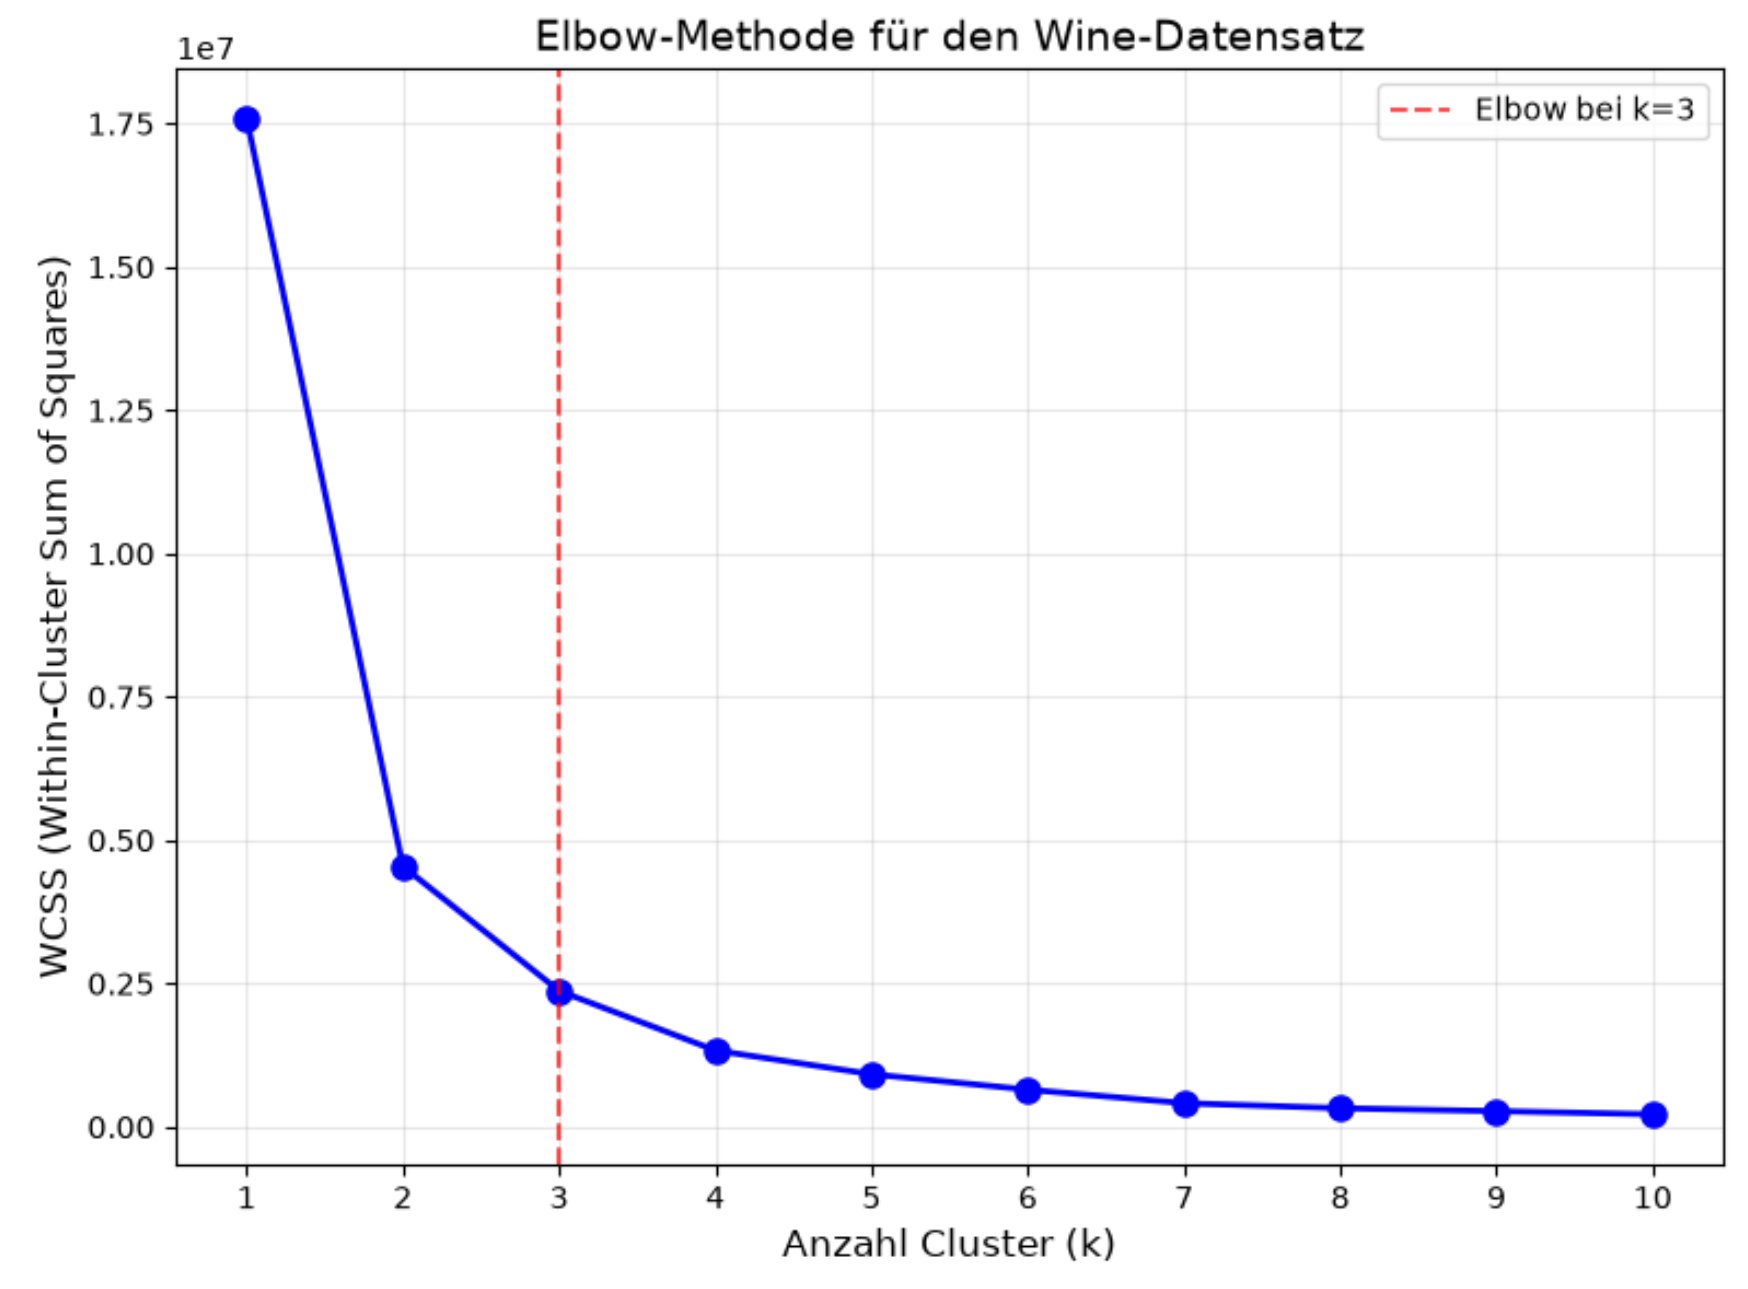
\includegraphics[width=0.9\textwidth]{./asset/image/Aufgabe3f.png}
    \caption{Elbow-Methode für den Wine-Datensatz (\textit{Quelle: Eigene Darstellung})}
    \label{fig:aufgabe3f}
\end{figure}

\subsection{Interpretation}

Die Elbow-Methode wird mit \texttt{KMeans} aus \texttt{sklearn.cluster} für \(k = 1\) bis \(10\) durchgeführt. Für jeden Wert von \(k\) wird der \acs{WCSS}-Wert (\textit{\texttt{inertia\_}}) berechnet und gespeichert.

Der Elbow-Plot zeigt, dass der \acs{WCSS}-Wert mit zunehmender Cluster-Anzahl \(k\) abnimmt. Der Abfall ist bis \(k = 3\) stark, danach flacht die Kurve deutlich ab. Der Knick (\textit{Elbow}) ist bei \(k = 3\) am deutlichsten erkennbar.

Die Elbow-Methode liefert somit \(k = 3\) als geeignete Cluster-Anzahl für den Wine-Datensatz. Dies ist plausibel, da der Datensatz aus drei verschiedenen Weinsorten besteht (\textit{wie aus den vorherigen Aufgaben bekannt}). Die natürliche Cluster-Struktur des Datensatzes wird durch die Elbow-Methode bestätigt.

\cleardoublepage

% ======================================= g =====================================

\section{Visualisierung der Clusterung mittels K-Means (g)}
\label{sec:3g}

\subsection{Aufgabenstellung}

Die Daten des Wine-Datensatzes werden mittels K-Means-Clustering mit der in Aufgabe 3f ermittelten Cluster-Anzahl (\textit{\(k = 3\)}) geclustert. Die Clusterung wird visualisiert.

\subsection{Lösung}

Das K-Means-Clustering wird mit \texttt{KMeans} aus \texttt{sklearn.cluster} für \(k = 3\) durchgeführt. Die Cluster-Zugehörigkeiten werden mit \texttt{fit\_predict()} berechnet und als neue Spalte \texttt{cluster} im \texttt{DataFrame} gespeichert. Zur Visualisierung wird ein Scatter-Plot der ersten beiden Hauptkomponenten (\textit{\acs{PCA}}) erstellt, um die Cluster in einem zweidimensionalen Raum darzustellen.

\lstinputlisting[
    language=Python,
    caption={K-Means-Clustering mit \(k = 3\) und Visualisierung},
    label={lst:aufgabe3g}
]{asset/code/Aufgabe3g.tex}

\paragraph{\textbf{Hinweis zur Visualisierung}}

Die Visualisierung der Cluster erfolgt mittels Hauptkomponentenanalyse (\textit{\acs{PCA}}), um die hochdimensionalen Daten (\textit{13 Features}) auf zwei Dimensionen zu reduzieren. Dies ermöglicht eine übersichtliche Darstellung der Cluster-Struktur. Alternativ könnten auch zwei besonders trennscharfe Features (\textit{\acs{z. B.} \texttt{proline} und \texttt{od280/od315\_of\_diluted\_wines}}) für die Visualisierung verwendet werden.

\subsection{Ausgabe}

Die Ausgabe zeigt die Visualisierung der drei Cluster im zweidimensionalen \acs{PCA}-Raum:

\begin{figure}[h]
    \centering
    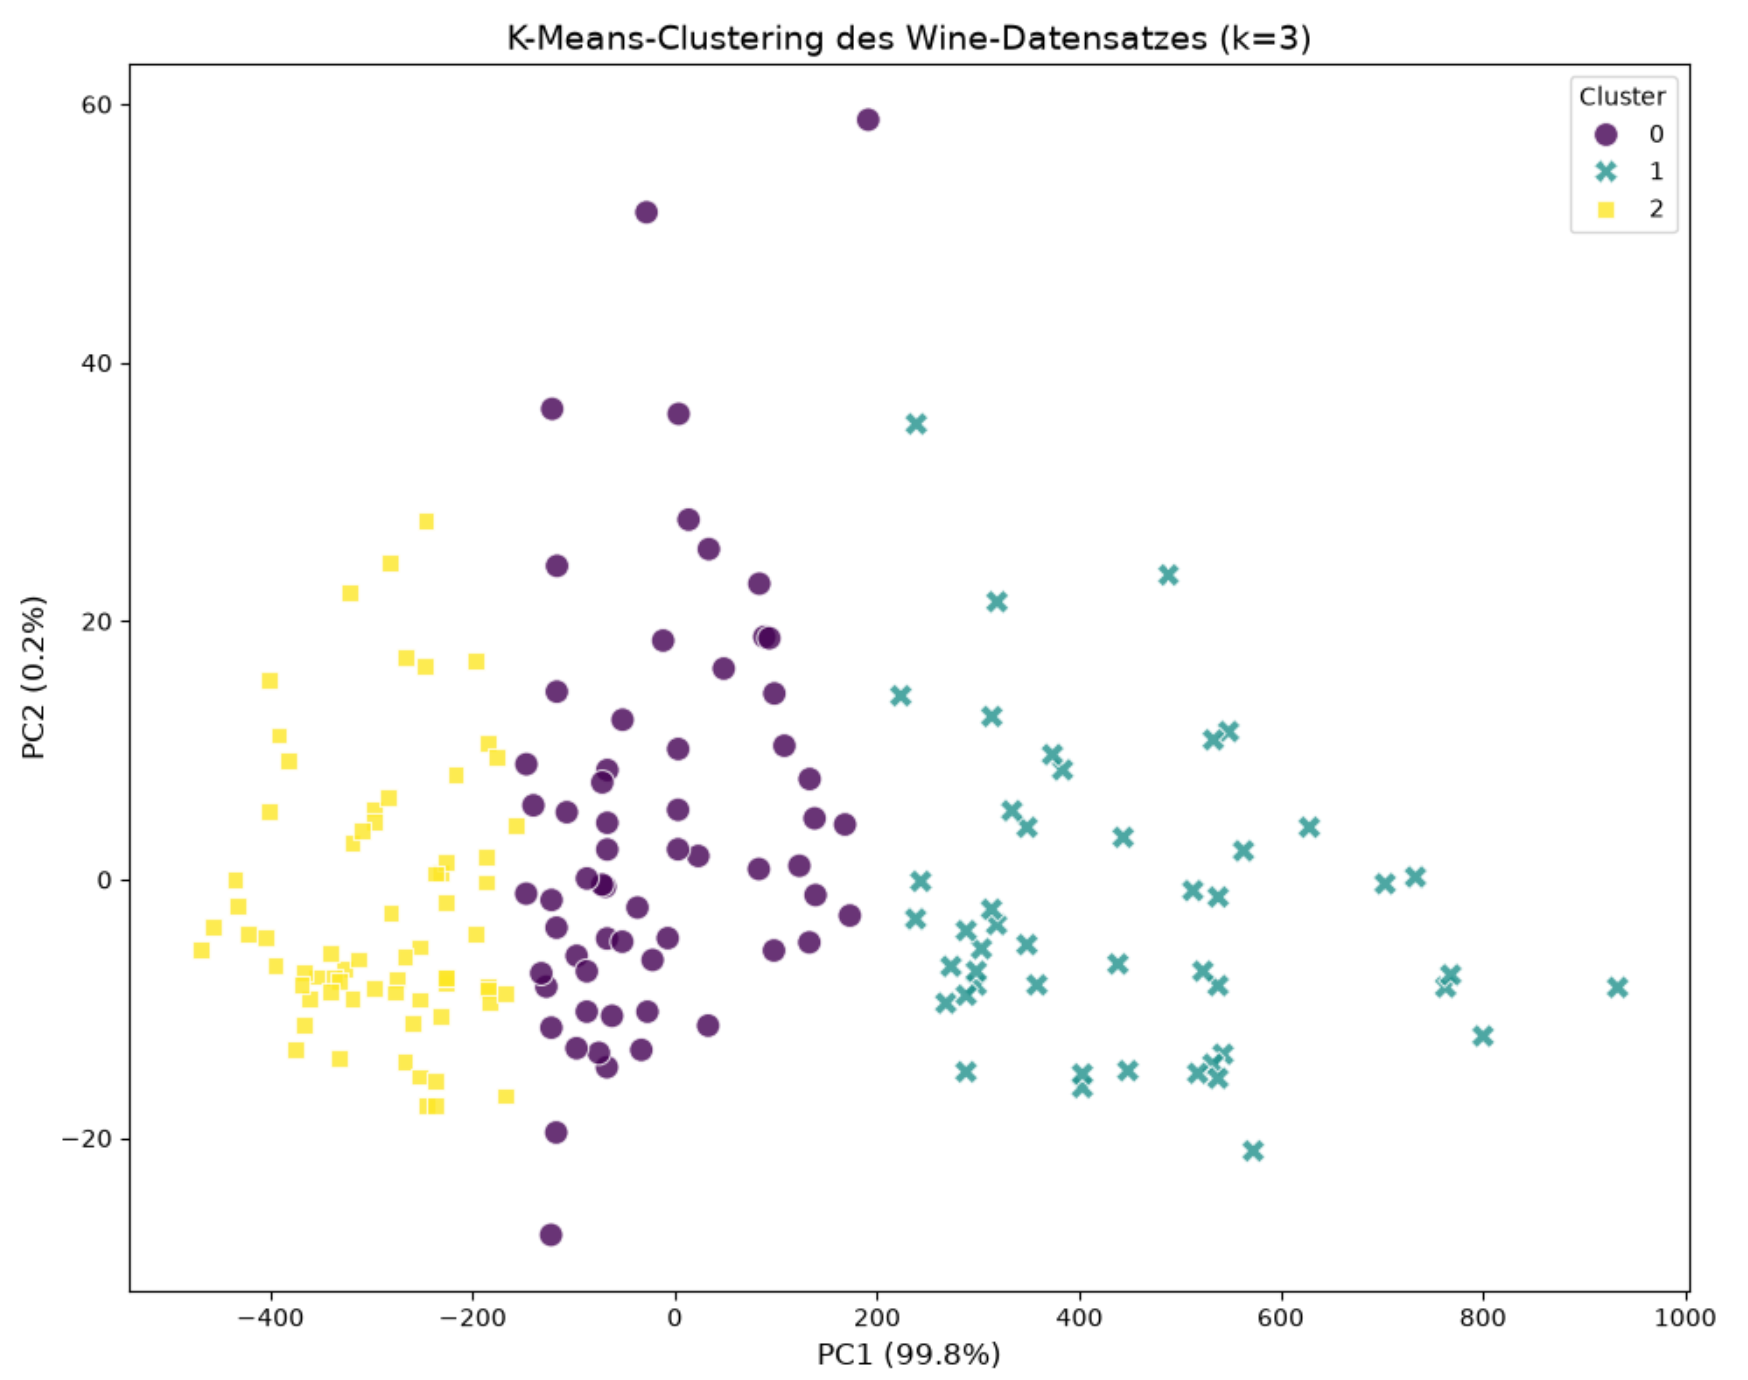
\includegraphics[width=0.9\textwidth]{./asset/image/Aufgabe3g.png}
    \caption{K-Means-Clustering des Wine-Datensatzes mit \(k = 3\) (\textit{Quelle: Eigene Darstellung})}
    \label{fig:aufgabe3g}
\end{figure}

\subsection{Interpretation}

Das K-Means-Clustering wird mit \texttt{KMeans(\textit{n\_clusters=3}, \textit{random\_state=42}, \textit{n\_init=10})} durchgeführt. Die Cluster-Zugehörigkeiten werden mit \texttt{fit\_predict()} berechnet und im \texttt{DataFrame} gespeichert.

Die Visualisierung mittels \acs{PCA} zeigt die drei Cluster als deutlich voneinander getrennte Gruppen. Die Cluster sind im zweidimensionalen Raum gut separiert, was die natürliche Cluster-Struktur des Wine-Datensatzes bestätigt. Die drei Cluster entsprechen den drei verschiedenen Weinsorten (\textit{class 0, 1, 2}).

Die \acs{PCA}-Reduktion von 13 Dimensionen auf 2 Hauptkomponenten ermöglicht eine übersichtliche Darstellung der Cluster-Struktur. Die erste Hauptkomponente (\textit{\acs{PC1}}) erklärt den größten Teil der Varianz und trennt die Cluster 0 und 1, während die zweite Hauptkomponente (\textit{\acs{PC2}}) die Cluster 1 und 2 weiter differenziert.

Die Visualisierung bestätigt, dass \(k = 3\) eine geeignete Cluster-Anzahl für den Wine-Datensatz ist.

\cleardoublepage

% ======================================= h =====================================

\section{Elbow-Methode nach Skalierung mit StandardScaler (h)}
\label{sec:3h}

\subsection{Aufgabenstellung}

Da die Größendordnungen der Spalten des Wine-Datensatzes unterschiedlich sind (\textit{wie in Aufgabe 3c gezeigt}), wird eine Skalierung der Daten mit dem \texttt{StandardScaler} durchgeführt. Anschließend wird die Elbow-Methode auf den skalierten Daten angewendet. Es wird ermittelt, welchen Wert \(k\) die Elbow-Methode für den skalierten Datensatz liefert und wie dieses Ergebnis bewertet wird.

\subsection{Lösung}

Zunächst werden die Daten mit \texttt{StandardScaler} aus \texttt{sklearn.preprocessing} skaliert. Der Skaler standardisiert die Daten, sodass jede Variable einen Mittelwert von 0 und eine Standardabweichung von 1 hat. Die skalierten Daten werden in einen \texttt{Pandas DataFrame} umgewandelt. Anschließend wird die Elbow-Methode auf den skalierten Daten für \(k = 1\) bis \(10\) durchgeführt.

\lstinputlisting[
    language=Python,
    caption={Elbow-Methode nach Skalierung mit StandardScaler},
    label={lst:aufgabe3h}
]{asset/code/Aufgabe3h.tex}

\paragraph{\textbf{Hinweis zur Skalierung}}

Die Skalierung mit \texttt{StandardScaler} ist für K-Means-Clustering empfehlenswert, da K-Means auf Distanzberechnungen basiert. Variablen mit großen Wertebereichen (\textit{wie \texttt{proline}}) würden sonst die Clusterbildung dominieren. Durch die Standardisierung erhalten alle Variablen das gleiche Gewicht.

\subsection{Ausgabe}

Die Ausgabe zeigt den Elbow-Plot für die skalierten Daten:

\begin{figure}[h]
    \centering
    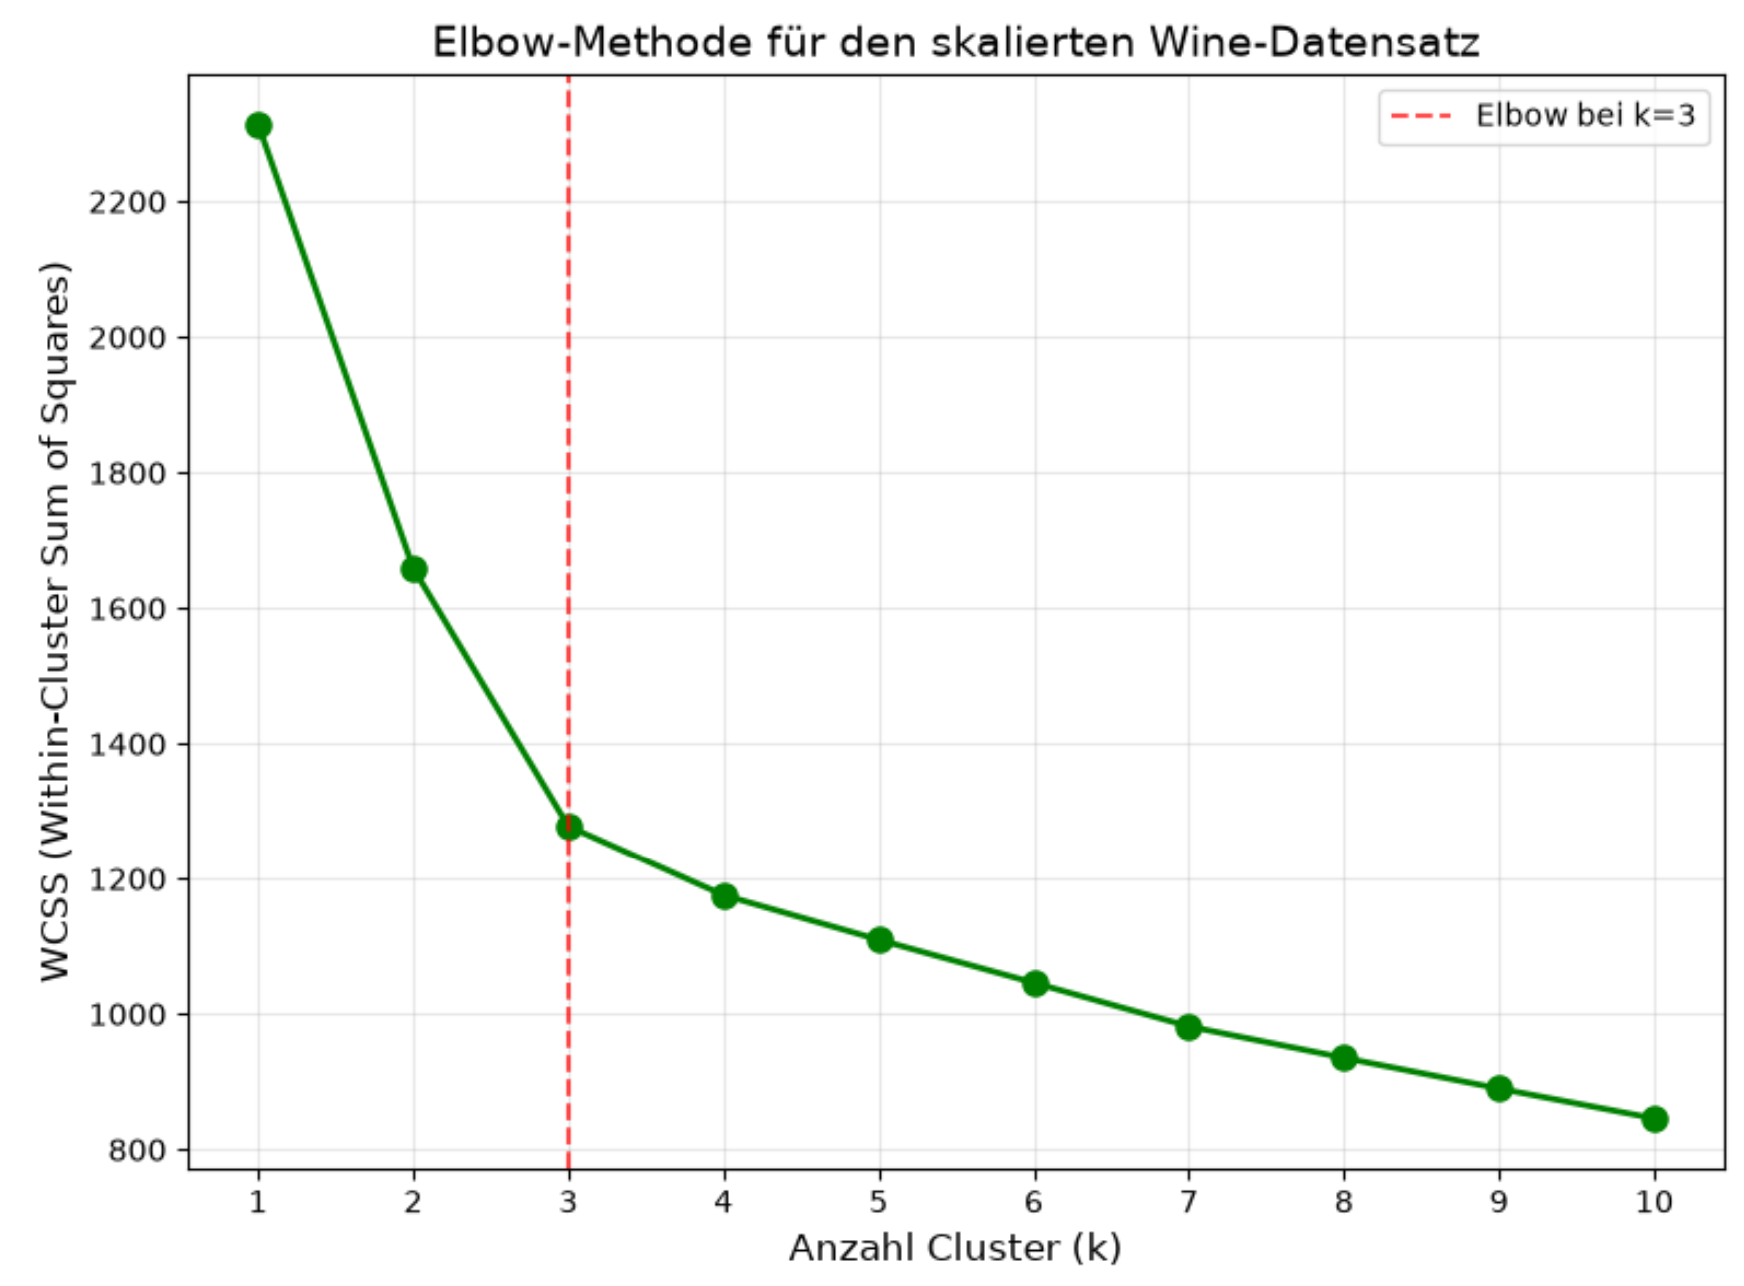
\includegraphics[width=0.9\textwidth]{./asset/image/Aufgabe3h.png}
    \caption{Elbow-Methode für den skalierten Wine-Datensatz (\textit{Quelle: Eigene Darstellung})}
    \label{fig:aufgabe3h}
\end{figure}

Die Elbow-Methode liefert für den skalierten Datensatz ebenfalls \(k = 3\) als geeignete Cluster-Anzahl.

\subsection{Interpretation}

Die Skalierung der Daten mit \texttt{StandardScaler} standardisiert alle 13 Variablen auf einen Mittelwert von 0 und eine Standardabweichung von 1. Dies ist für K-Means-Clustering essenziell, da der Algorithmus auf euklidischen Distanzen basiert und Variablen mit großen Wertebereichen sonst einen unverhältnismäßig großen Einfluss auf die Clusterbildung hätten.

Der Elbow-Plot für die skalierten Daten zeigt einen noch deutlicheren Knick bei \(k = 3\) als bei den unskalierten Daten. Der \acs{WCSS}-Wert fällt bis \(k = 3\) stark ab, danach flacht die Kurve deutlich ab. Der Elbow bei \(k = 3\) ist nun klarer ausgeprägt.

\textbf{Bewertung des Ergebnisses:}

Das Ergebnis \(k = 3\) nach der Skalierung bestätigt das Ergebnis aus Aufgabe 3f. Die Tatsache, dass die Elbow-Methode sowohl vor als auch nach der Skalierung \(k = 3\) liefert, spricht für die Robustheit dieses Ergebnisses. Die Skalierung führt zu einem klareren Elbow und damit zu einer eindeutigeren Entscheidung für \(k = 3\).

Die drei Cluster entsprechen den drei verschiedenen Weinsorten des Datensatzes. Das Ergebnis zeigt, dass der Wine-Datensatz eine natürliche Cluster-Struktur mit drei Gruppen aufweist. Die Skalierung war für die Analyse nicht zwingend erforderlich, da bereits die unskalierten Daten den Elbow bei \(k = 3\) zeigten, sie verbessert jedoch die Interpretierbarkeit und Robustheit des Ergebnisses.

% ==============================================================================
% =============================== Ende Aufgabe 3 ===============================
% ==============================================================================